\section{Two-insertion processes}\label{sec:10.8}

A dark photon of \SI{100}{keV} that meets an electron in silicon is more likely to scatter off it than to be absorbed. It leaves as an ordinary photon of \SI{91.8}{keV}, and the electron recoils with the remaining \SI{8.2}{keV}. This is dark Compton scattering, and above about \SI{55}{keV} it is the main way a silicon detector registers a dark photon. Its amplitude carries two insertions of a field: one of the dark photon and one of the photon. A complex scalar that couples quadratically to the electrons, through $\phi^\dagger\phi$, is a second example. It cannot be absorbed singly, since the coupling destroys a particle only together with an antiparticle, and the target absorbs the pair, the energy $2m_\phi$ and the momentum of both. Each process asks the crystal for more than the single row of \cref{sec:10.7}.

\subsection{Second-order transition operator}\label{sec:10.8-rate}

To second order in the interaction $H' = H_{\mathrm{int}}$, the Lippmann--Schwinger series \cref{eq:2.4-LS} gives $T_{fi} = H'_{fi} + \sum_mH'_{fm}H'_{mi}/(E_i - E_m + \ii0^+)$, and the rate is $2\pi|T_{fi}|^2\delta(E_f - E_i)$ (\cref{eq:2.4-golden2}). A field can enter $T_{fi}$ twice in two ways. In the first, one term of $H_{\mathrm{int}}$ is already quadratic in the field and linear in a target operator, so that both insertions sit at one vertex. The first-order term of $T$ then removes two quanta at once, and the target answers with one of its rows $O_a$ at the total momentum and energy of the pair. The rate needs only the response matrix $S_{ab}$ of \cref{eq:8.2-rate}. In the second way, each insertion comes with its own target operator, and the second-order term of $T$ joins them through the target propagator. With insertions $a$ and $b$ that bring $(\vect{k}_1, \omega_1)$ and $(\vect{k}_2, \omega_2)$, the target sees the effective operator
\begin{equation}
  T^{(2)}_{ab} = O_b(\vect{k}_2)\,\frac{1}{E_i + \omega_1 - H_0 + \ii0^+}\,O_a(\vect{k}_1) + O_a(\vect{k}_1)\,\frac{1}{E_i + \omega_2 - H_0 + \ii0^+}\,O_b(\vect{k}_2) ,
  \label{eq:10.8-T2}
\end{equation}
the two time orderings of \cref{eq:2.4-orderings}, and the rate is the response of $T^{(2)}_{ab}$, a four-point function of the target operators, at $(\vect{k}_1 + \vect{k}_2, \omega_1 + \omega_2)$. When neither denominator can vanish, because $\omega_1$ and $\omega_2$ lie below every excitation that $O_a$ and $O_b$ reach, $T^{(2)}_{ab}$ is to leading order a static polarizability of the target, and the four-point function collapses to a two-point function. A vector field coupled to the electron current brings a contact term of its own, the seagull $e^2\vect{A}^2/2m_e$ of the electron Hamiltonian. When the frequencies lie far above the binding energies of the electrons, the second-order terms are small against it, and the seagull alone gives the Thomson limit. Dark Compton scattering is this case (\cref{sec:10.8-compton}). A coupling that has both a contact term and two linear ones gives amplitudes of both kinds, and their interference needs a three-point response of the target, linear in a quadratic response function (\cref{sec:10.8-open}).

\subsection{Pair absorption}\label{sec:10.8-pair}

Take a complex scalar $\phi$ of mass $m_\phi$, whose particles and antiparticles are equally abundant, each with the number density $\rho_\chi/2m_\phi$. Bauer, Perez-Soler and Shergold write its lowest couplings to electrons, in Hamiltonian form, as~\cite[Eq.~(3)]{bauer2026dark}
\begin{equation}
  H_{\mathrm{int}} = \int\dd^3x\,\Bigl[m_e\,\phi^\dagger\phi\;\bar\psi\bigl(G_{\mathrm{S}} + \ii G_{\mathrm{P}}\gamma^5\bigr)\psi
  + \ii\bigl(\phi^\dagger\overleftrightarrow{\partial}_{\!\mu}\phi\bigr)\,\bar\psi\gamma^\mu\bigl(G_{\mathrm{V}} + G_{\mathrm{A}}\gamma^5\bigr)\psi\Bigr] ,
  \label{eq:10.8-Hpair}
\end{equation}
with $\phi^\dagger\overleftrightarrow{\partial}_{\!\mu}\phi = \phi^\dagger\partial_\mu\phi - (\partial_\mu\phi^\dagger)\phi$ and four real couplings of dimension eV$^{-2}$, for scalar, pseudoscalar, vector and axial-vector electron bilinears. They are dimension-six operators, of order $\Lambda_{\mathrm{NP}}^{-2}$ for a new-physics scale $\Lambda_{\mathrm{NP}}$, and we quote rates at $G = G_{\mathrm{F}}$, the Fermi constant. To first order in the couplings the interaction Hamiltonian is minus the interaction Lagrangian, derivative terms included. Each operator is quadratic in $\phi$ and linear in the electrons, so pair absorption is a contact process of the first kind.

\emph{The rate.} Quantize $\phi$ in the box. The field operator removes a particle of momentum $\vect{p}$ with the factor $\ee^{\ii\vect{p}\cdot\vect{x} - \ii E t}/\sqrt{2E\Vol}$ and $\phi^\dagger$ removes an antiparticle of momentum $\bar{\vect{p}}$ with $\ee^{\ii\bar{\vect{p}}\cdot\vect{x} - \ii\bar Et}/\sqrt{2\bar E\Vol}$, with $E$ and $\bar E$ their energies. Removing both from $\phi^\dagger\phi$ leaves the plane wave $\ee^{\ii(\vect{p} + \bar{\vect{p}})\cdot\vect{x}}/(\Vol\sqrt{4E\bar E})$. In $\ii\phi^\dagger\overleftrightarrow{\partial}_{\!\mu}\phi$ the derivatives bring down $-\ii p_\mu$ and $-\ii\bar p_\mu$ with opposite signs, and the same plane wave comes with the factor $(p - \bar p)_\mu$. Every operator of \cref{eq:10.8-Hpair} therefore acts on the target as a row at the total momentum of the pair, $\vect{q} = \vect{p} + \bar{\vect{p}}$, with a coefficient $g^{\phi\phi}_a$ per unit pair amplitude. The coefficients are $m_eG_{\mathrm{S}}$ and $m_eG_{\mathrm{P}}$ against the bilinears $\bar\psi\psi$ and $\bar\psi\ii\gamma^5\psi$, and $G_{\mathrm{V}}(p - \bar p)^\mu$ and $G_{\mathrm{A}}(p - \bar p)^\mu$ against the vector and axial currents. The golden rule, summed over final states, turns $\sum_f2\pi|\langle f|O_b(\vect{q})|i\rangle|^2\delta(\omega - E_f + E_i)$ into $\Vol S_{bb}(\vect{q}, \omega)$, as in \cref{eq:8.2-abs}, and one pair in the box is absorbed at the rate $\sum_{ab}g^{\phi\phi*}_a g^{\phi\phi}_bS_{ab}/(4E\bar E\Vol)$. The box holds $\Vol^2$ times $(\rho_\chi/2m_\phi)^2$ pairs, distributed over the two velocities with the laboratory distribution $f_\chi$ of \cref{sec:1.2}. The number of pairs absorbed per unit time and volume is
\begin{equation}
  \frac{\varGamma_{\mathrm{pair}}}{\Vol} = \Bigl(\frac{\rho_\chi}{2m_\phi}\Bigr)^2\int\dd^3v\,\dd^3\bar v\,f_\chi(\vect{v})f_\chi(\bar{\vect{v}})\,
  \frac{\sum_{ab}g^{\phi\phi*}_a g^{\phi\phi}_b\,S_{ab}(\vect{p} + \bar{\vect{p}},\,E + \bar E)}{4E\bar E} ,
  \label{eq:10.8-pair}
\end{equation}
with $\vect{p} = m_\phi\vect{v}$, $\bar{\vect{p}} = m_\phi\bar{\vect{v}}$ and $E + \bar E = 2m_\phi + K_{\mathrm{pair}}$, where $K_{\mathrm{pair}} = \frac12m_\phi(v^2 + \bar v^2)$ is the kinetic energy of the pair. The event rate per unit target mass is $\varGamma_{\mathrm{pair}}/(\Vol\rho_T)$. This is the golden rule and phase-space measure of Bauer and collaborators~\cite[Eqs.~(5) and (7)]{bauer2026dark} with $S_{ab}$ in place of a single atomic transition. Their truncated Gaussian momentum distribution of each species~\cite[Eq.~(8)]{bauer2026dark}, written per degree of freedom, integrates to the number density $\rho_\chi/2m_\phi$ used here, so their rates equal ours at the same density. Their rates assume $\rho_\chi = \SI{0.39}{GeV.cm^{-3}}$ and scale as $\rho_\chi^2$, so they are larger than at the \SI{0.3}{GeV.cm^{-3}} of \cref{sec:1.2} by $(0.39/0.3)^2 = 1.69$.

The response is sampled close to a single point. The total momentum is at most $2m_\phi v_{\mathrm{max}} = 5.3\times10^{-3}\,m_\phi$, and the pair's kinetic energy has the mean $\bar K_{\mathrm{pair}} = m_\phi\langle v^2\rangle = 1.60\times10^{-6}\,m_\phi$ in the laboratory, for the halo of \cref{sec:1.2} ($\langle v^2\rangle^{1/2} = \SI{379}{km/s}$), with a spread of half that. For an electronic transition at $2m_\phi = \SI{10}{eV}$ the momentum times the lattice constant is $qa < 10^{-4}$. Wherever $S_{ab}$ is smooth on the scale $\bar K_{\mathrm{pair}}$ in energy, it can be taken at $(\vect{0}, 2m_\phi)$, and
\begin{equation}
  \frac{\varGamma_{\mathrm{pair}}}{\Vol} = \Bigl(\frac{\rho_\chi}{2m_\phi}\Bigr)^2\,\frac{\sum_{ab}\langle g^{\phi\phi*}_a g^{\phi\phi}_b\rangle\,S_{ab}(0, 2m_\phi)}{4m_\phi^2} ,
  \label{eq:10.8-contact}
\end{equation}
with the average over the two velocities left only on the coefficients. Pair absorption is single absorption at the energy $2m_\phi$, with a tensor of coefficients that may depend on the velocities. Which rows the four couplings reach, and with what coefficients, follows from the non-relativistic reduction of the electron bilinears, which \cref{sec:1.4,sec:8.1-absorption} have done for linear couplings. The reduction does not care whether the field multiplying a bilinear is $\phi$ or $\phi^\dagger\phi$.

\emph{Scalar.} By \cref{eq:8.1-scalar}, $\bar\psi\psi$ is $n_e - \mathcal{T}_e/m_e$ at low energy. The density row connects different states only at order $q$, and the kinetic row survives at $\vect{q} = 0$, as for a single scalar (\cref{sec:10.7-scalar}). With $g^{\phi\phi} = m_eG_{\mathrm{S}}$ against $\mathcal{T}_e/m_e$, \cref{eq:10.8-contact} gives $(\rho_\chi/2m_\phi)^2G_{\mathrm{S}}^2S_{\mathcal{T}\mathcal{T}}(0, 2m_\phi)/4m_\phi^2$. Compare it with \cref{eq:10.7-scalar} for a scalar of mass $2m_\phi$ and coupling $g_{\phi ee}$, absorbed at the rate $g_{\phi ee}^2S_{\mathcal{T}\mathcal{T}}(0, 2m_\phi)/(4m_\phi m_e^2)$ per particle. The pair rate per unit volume equals the rate of a scalar of mass $2m_\phi$ at the number density $\rho_\chi/2m_\phi$ when
\begin{equation}
  g_{\phi ee}^2 \;\to\; g_{\mathrm{eff}}^2 = \frac{\rho_\chi}{2m_\phi}\,\frac{m_e^2G_{\mathrm{S}}^2}{m_\phi} .
  \label{eq:10.8-geff}
\end{equation}
The rate per unit volume grows as $\rho_\chi^2/m_\phi^4$ at fixed response, and this is what makes pair absorption interesting at small masses.

\emph{Pseudoscalar.} The non-relativistic form of $\bar\psi\ii\gamma^5\psi$ times a field is \cref{eq:1.4-alp}, with $g_{aee}\phi$ replaced by $m_eG_{\mathrm{P}}\phi^\dagger\phi$. It has two terms. The spin-density term carries the gradient of the field, which on the pair is $\ii\vect{q}$, and is negligible. The spin-current term carries its time derivative, which on the pair is $-\ii(E + \bar E) \simeq -2\ii m_\phi$, not the momentum. The pseudoscalar pair is therefore absorbed through the axioelectric row $\mathcal{J}_e$ of \cref{sec:10.7-alp}, with the coefficient $2m_\phi G_{\mathrm{P}}$ in place of $g_{aee}m_\phi/m_e$, and without any velocity suppression. With $S_{\mathcal{J}\mathcal{J}} = \frac34S_{jj}$ and $S_{jj}(0, \omega) = 2\omega\sigma_1/e^2$ (\cref{sec:10.7-alp}),
\begin{equation}
  \frac{\varGamma_{\mathrm{pair}}}{\Vol} = \Bigl(\frac{\rho_\chi}{2m_\phi}\Bigr)^2G_{\mathrm{P}}^2\,S_{\mathcal{J}\mathcal{J}}(0, 2m_\phi) = \Bigl(\frac{\rho_\chi}{2m_\phi}\Bigr)^2\,\frac{3m_\phi\,G_{\mathrm{P}}^2}{e^2}\,\sigma_1(2m_\phi) ,
  \label{eq:10.8-P}
\end{equation}
which is \cref{eq:10.7-alp} at the mass $2m_\phi$ with $g_{aee}^2 \to g_{\mathrm{eff}}^2$ of \cref{eq:10.8-geff}, $G_{\mathrm{S}}$ replaced by $G_{\mathrm{P}}$. It inherits the caveats of the axioelectric row: the measured $\sigma_1$ belongs to singlet pairs and the row creates triplets, and spin--orbit coupling spoils the factor $\frac34$.

\emph{Vector.} The coefficient $(p - \bar p)^\mu$ is orthogonal to the total four-momentum of the pair, exactly: $(p + \bar p)\cdot(p - \bar p) = E^2 - \bar E^2 - \vect{p}^2 + \bar{\vect{p}}^2 = m_\phi^2 - m_\phi^2 = 0$. A dark photon of four-momentum $k$ couples to the electron current through its polarization $\epsilon^\mu$, with $k\cdot\epsilon = 0$. The vector pair is therefore a dark photon of four-momentum $p + \bar p$, mass close to $2m_\phi$ and polarization $(p - \bar p)^\mu$, whose length squared is $-(p - \bar p)^2 = |\vect{p} - \bar{\vect{p}}|^2 - (E - \bar E)^2 \simeq m_\phi^2|\vect{v} - \bar{\vect{v}}|^2$, coupled with $G_{\mathrm{V}}$ in place of $\zeta e$. Since it couples to the electron current, it mixes with the photon of the medium as a dark photon does, and the in-medium chain of \cref{sec:10.7-darkphoton} applies. A dark photon at rest is absorbed at $\zeta^2\omega L(\omega)$, which by \cref{eq:8.2-abs} is $(\zeta e)^2/2\omega$ times the screened current response along a unit polarization; that response is therefore $2\omega^2L/e^2$, and
\begin{equation}
  \frac{\varGamma_{\mathrm{pair}}}{\Vol} = \Bigl(\frac{\rho_\chi}{2m_\phi}\Bigr)^2\,\frac{2G_{\mathrm{V}}^2}{e^2}\,m_\phi^2\,\langle|\vect{v} - \bar{\vect{v}}|^2\rangle\,L(2m_\phi) ,
  \label{eq:10.8-V}
\end{equation}
with corrections of order $v^2$ from the difference between longitudinal and transverse polarizations (\cref{eq:10.7-TL}). The relative velocity is the same in every frame, and for the halo of \cref{sec:1.2} $\langle|\vect{v} - \bar{\vect{v}}|^2\rangle^{1/2} = \SI{402}{km/s}$, close to $\sqrt3v_0 = \SI{412}{km/s}$ for a Maxwellian without the escape cut. The derivative coupling brings the factor $\langle|\vect{v} - \bar{\vect{v}}|^2\rangle = 1.8\times10^{-6}$.

\emph{Axial vector.} The space components of $\bar\psi\gamma^\mu\gamma^5\psi$ reduce to twice the spin density $\vect{s}_e$, and the time component to a spin--velocity term like $\mathcal{J}_e$. The time component comes with $E - \bar E = O(m_\phi v^2)$. The space components come with $\vect{p} - \bar{\vect{p}} = O(m_\phi v)$, but they act through $\vect{s}_e(\vect{q})$, and without spin--orbit coupling or magnetic order $\vect{s}_e(0)$ is the total spin, which commutes with the Hamiltonian and connects no two different states. Both amplitudes are therefore of order $v^2$, and the rate of order $v^4$. The spin-density row comes back at $\vect{q} = 0$ only where the target has spin-split levels: the Zeeman sublevels of an atom in a field, which Bauer and collaborators use in hydrogen~\cite[Eq.~(23)]{bauer2026dark}, or the magnon of an ordered magnet (\cref{sec:14.3}). Their squared amplitude for the spin flip, $G_{\mathrm{A}}^2$ times the square of the relative velocity transverse to the field over four, is the integrand of \cref{eq:10.8-pair} with $g^{\phi\phi,\mu} = G_{\mathrm{A}}(p - \bar p)^\mu$ against $2\vect{s}_e$ and the normalization $1/4E\bar E$.

\Cref{fig:10-twoins}a shows the three unsuppressed rates of silicon at $G = G_{\mathrm{F}}$. They are small. At $m_\phi = \SI{5}{eV}$, where the pair deposits \SI{10}{eV}, the kinetic row of the pseudopotential model of \cref{sec:10.7-scalar} gives $1.6\times10^{-12}$ events per kilogram-year, the pseudoscalar $4.0\times10^{-17}$ and the vector $4.7\times10^{-24}$. Three events in a kilogram-year would need $G_{\mathrm{S}} = 1.4\times10^6\,G_{\mathrm{F}}$, an interaction stronger than the weak one by a factor of a million, at a scale $\Lambda_{\mathrm{NP}} \approx \SI{0.25}{GeV}$. In the language of \cref{eq:10.8-geff}, $G = G_{\mathrm{F}}$ at \SI{5}{eV} corresponds to $g_{\mathrm{eff}} = 1.3\times10^{-21}$. The scaling $\rho_\chi^2/m_\phi^4$ favors much lighter particles, and this is where Bauer and collaborators find pair absorption competitive: spin flips of atoms at \si{\micro eV} energies, whose splitting a magnetic field tunes. A crystal has no electronic transition there. The density row of the scalar, which the kinetic row dwarfs by a factor of 50 at \SI{10}{eV}, matches it near the plasmon, as for single absorption (\cref{sec:10.7-scalar}).

\begin{figure}[tbp]
  \centering
  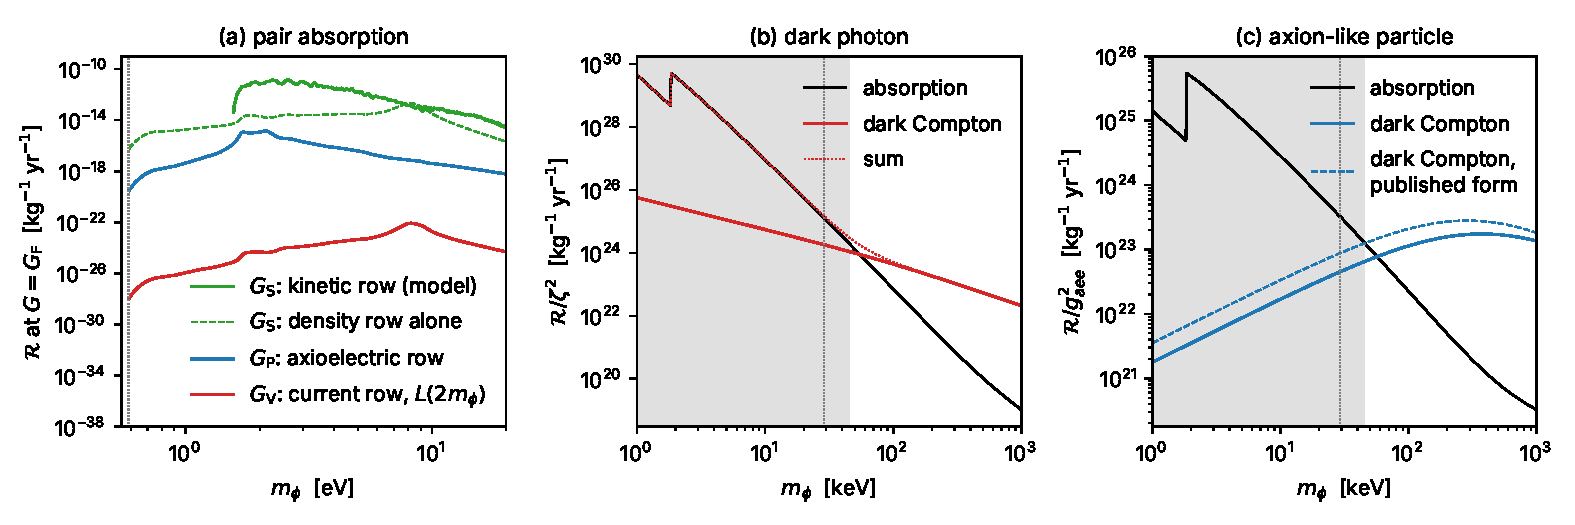
\includegraphics[width=\linewidth]{figures/ch10/fig10_7.pdf}
  \caption{Two-insertion rates of bosonic dark matter in silicon per kilogram-year, with $\rho_\chi = \SI{0.3}{GeV.cm^{-3}}$, $\rho_T = \SI{2.33}{g.cm^{-3}}$ and the halo of \cref{sec:1.2}. (a) Pair absorption of a complex scalar of mass $m_\phi$ at couplings $G = G_{\mathrm{F}}$, \cref{eq:10.8-contact}. Scalar through the kinetic row in the empirical-pseudopotential model of \cref{sec:10.7-scalar}, which has its own vertical gap at \SI{3.12}{eV} and is a model, not a prediction (solid green). Scalar through the density row alone with $\langle q^2\rangle^{1/2} = 2.14\times10^{-3}\,m_\phi$ and the measured loss function (dashed). Pseudoscalar, \cref{eq:10.8-P}, and vector, \cref{eq:10.8-V}, from the measured optical constants of float-zone silicon at \SI{300}{K}~\cite{franta2017temperature}, spliced at \SI{40}{eV} to atomic scattering factors~\cite{henke1993xray}. Dotted: $2m_\phi$ at the excitonic edge of cold silicon, \SI{1.1728}{eV} with $\Eg(0) = \SI{1.1692}{eV}$; the \SI{300}{K} data are wrong within tens of meV of it (\cref{sec:10.7-edge}). (b) Dark photon: absorption, \cref{eq:10.7-dp} (black; from the optical constants below \SI{29}{keV}, dotted line, and from the photoelectric cross section of the XCOM tables (the photon cross-section database of the National Institute of Standards and Technology)~\cite{berger2010xcom} above, with $\varepsilon = 1$), and dark Compton scattering on all 14 electrons, \cref{eq:10.8-compton} (red). (c) Axion-like particle: absorption, \cref{eq:10.7-alp} (black), and dark Compton scattering, \cref{eq:10.8-alpC} (blue). Gray in (b) and (c): $m_\phi < \SI{45}{keV}$, where the electron recoil $\omega_{\mathrm{C}}$ falls below the K-shell binding of \SI{1.84}{keV} and counting all 14 electrons as free overstates the Compton rate.}
  \label{fig:10-twoins}
\end{figure}

The reduction to \cref{eq:10.8-contact} assumes a smooth response. A target with a sharp line at $\Delta E$ resolves the kinetic energy of the pair instead: the rate is spread over $2m_\phi$ between $\Delta E - 4\bar K_{\mathrm{pair}}$ and $\Delta E$, and the peak it reaches depends on how the width of the line compares with $\bar K_{\mathrm{pair}}$. This is the regime of the atomic transitions of Ref.~\cite{bauer2026dark}, whose line shape follows the kinetic-energy distribution of the pair. In silicon the absorption continua vary on scales of meV, and \cref{eq:10.8-contact} holds; only a line narrower than $\bar K_{\mathrm{pair}}$, about \SI{1.6}{\micro eV} at $m_\phi = \SI{1}{eV}$, would resolve the kinetic energy of the pair. \Cref{lim:10.8a} shows where the reduction fails.

\begin{limitbox}[Pair absorption][lim:10.8a]
Pair absorption as single absorption at $\omega = 2m_\phi$ and $\vect{q} \to 0$, \cref{eq:10.8-contact}, with the constant coefficients $m_eG_{\mathrm{S}}$, $m_eG_{\mathrm{P}}$ and the velocity-dependent $G_{\mathrm{V,A}}(p - \bar p)^\mu$~\cite[Eqs.~(3) and (5)--(8)]{bauer2026dark}.
\par\smallskip
{\centering
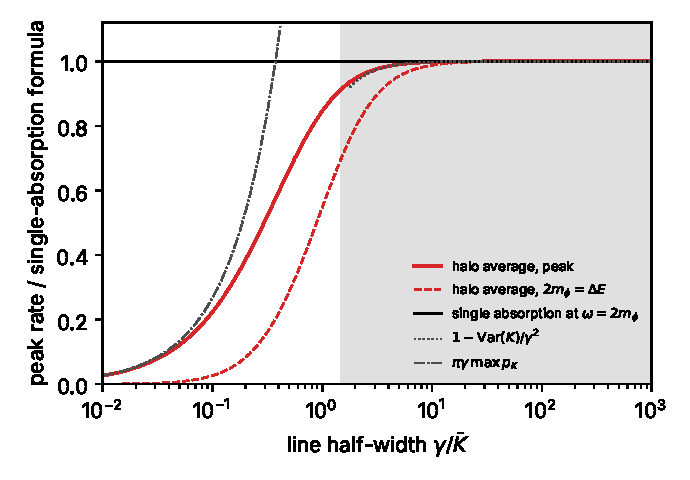
\includegraphics[width=0.72\linewidth]{figures/ch10/limit10_8a.pdf}
\captionof{figure}{Peak absorption rate of a model target with one Lorentzian line of half-width $\gamma$, as the halo average of \cref{eq:10.8-pair} over the pair kinetic energy $K_{\mathrm{pair}}$ (red), divided by the single-absorption formula \cref{eq:10.8-contact} (black), against $\gamma/\bar K_{\mathrm{pair}}$ with $\bar K_{\mathrm{pair}} = m_\phi\langle v^2\rangle = 1.60\times10^{-6}\,m_\phi$. Solid red: peak over the detuning $\Delta E - 2m_\phi$; dashed: at $2m_\phi = \Delta E$. Dotted: the leading correction for broad lines, $1 - \mathrm{Var}(K_{\mathrm{pair}})/\gamma^2$ with $\mathrm{Var}(K_{\mathrm{pair}}) = 0.253\,\bar K_{\mathrm{pair}}^2$; dash-dotted: the narrow-line limit $\pi\gamma\max p_K$, with $p_K$ the distribution of $K_{\mathrm{pair}}$, which the formula of Ref.~\cite{bauer2026dark} for a discrete transition reproduces. Halo of \cref{sec:1.2}, $2\times10^6$ velocity pairs; the dependence on $\vect{q}$ is dropped ($qa < 10^{-4}$). Gray: $\gamma \ge 1.5\,\bar K_{\mathrm{pair}}$, peak within \SI{10}{\percent} of the formula.}\label{fig:10-pair-limit}
\par}
\smallskip
For a line narrower than about $\bar K_{\mathrm{pair}}$, \SI{1.6}{\micro eV} at $m_\phi = \SI{1}{eV}$, the deposited energy follows the kinetic-energy distribution of the pair, and the formula overestimates the peak by $\bar K_{\mathrm{pair}}/\gamma$ up to a factor of order one.
\end{limitbox}

The pair-absorption rates need nothing that single absorption does not already compute: the absorption tables of the charge-like rows and the spin responses at $(\vect{q} \simeq 0, 2m_\phi)$, with the velocity moments of the vector and axial coefficients taken over two copies of the halo.

\subsection{Dark Compton scattering}\label{sec:10.8-compton}

A dark photon couples to the electrons as a photon does, with $e$ replaced by $\zeta e$ (\cref{sec:1.4}). An electron in the field of both therefore sees the total vector potential $\vect{A} + \zeta\vect{A}'$, and its Hamiltonian is $(\vect{p} + e\vect{A} + \zeta e\vect{A}')^2/2m_e$ plus the Pauli term. Expanded, it has the two linear couplings $(e/m_e)\vect{A}\cdot\vect{p}$ and $(\zeta e/m_e)\vect{A}'\cdot\vect{p}$, symmetrized, and a seagull that contains both fields at one point, $(\zeta e^2/m_e)\,\vect{A}\cdot\vect{A}'$. Absorbing a dark photon of polarization $\hat{\vect{e}}$ and emitting a photon of momentum $\vect{k}_\gamma$, energy $\omega_\gamma = |\vect{k}_\gamma|$ and polarization $\hat{\vect{e}}_\gamma$ is a process with two insertions. The seagull does it at first order, and the linear couplings at second order through \cref{eq:10.8-T2}. Per unit amplitude of each field, the target sees the transition operator
\begin{equation}
  T^{\mathrm{C}} = \frac{\zeta e^2}{m_e}\,(\hat{\vect{e}}\cdot\hat{\vect{e}}_\gamma^*)\,n_e(\vect{q})
  + \zeta e^2\Bigl[\hat{\vect{e}}_\gamma^*\cdot\vect{j}_e\,\frac{1}{E_i + m_\phi - H_0}\,\hat{\vect{e}}\cdot\vect{j}_e
  + \hat{\vect{e}}\cdot\vect{j}_e\,\frac{1}{E_i - \omega_\gamma - H_0}\,\hat{\vect{e}}_\gamma^*\cdot\vect{j}_e\Bigr] ,
  \label{eq:10.8-TC}
\end{equation}
with the momentum transfer $\vect{q} = \vect{p}_\phi - \vect{k}_\gamma \simeq -\vect{k}_\gamma$ and the current rows $\vect{j}_e$ at the momenta of their own fields. Both fields carry the factor $1/\sqrt{2\omega \Vol}$ of a quantum of energy $\omega$, as in \cref{eq:8.2-abs}. Summed over the momenta and polarizations of the photon, the golden rule gives the rate per dark photon
\begin{equation}
  \varGamma = \int\frac{\dd^3k_\gamma}{(2\pi)^3\,2\omega_\gamma}\,\frac{1}{2m_\phi}\sum_{\hat{\vect{e}}_\gamma}S_{T^{\mathrm{C}}T^{\mathrm{C}}}(\vect{q},\, m_\phi - \omega_\gamma) ,
  \label{eq:10.8-CS}
\end{equation}
averaged over the three polarizations $\hat{\vect{e}}$ of the dark photon. The target takes the energy $\omega = m_\phi - \omega_\gamma$ and the momentum $\vect{q}$, whose size is close to $m_\phi$. A dark photon of \SI{100}{keV} probes the electrons at $|\vect{q}| = \SI{92}{keV}$, or \SI{47}{\angstrom^{-1}}, far beyond every reciprocal-lattice vector and every inverse orbital radius except those of the innermost shells.

\emph{The Thomson limit.} For a free electron at rest both second-order terms vanish. If the dark photon is absorbed first, its vertex $\hat{\vect{e}}\cdot\vect{p}$ acts on an electron at rest, with $\vect{p}_\phi$ negligible. If the photon is emitted first, its vertex is $\hat{\vect{e}}_\gamma^*\cdot(\vect{p}_i + \vect{p}_m)/2 = -\hat{\vect{e}}_\gamma^*\cdot\vect{k}_\gamma/2 = 0$, since the photon is transverse. Only the seagull remains, and $S_{nn}(\vect{q},\omega) = 2\pi\nd_e\,\delta(\omega - q^2/2m_e)$ for electrons at rest. For $m_\phi \ll m_e$ each electron then scatters the dark photon with the cross section $\zeta^2\sigma_{\mathrm{Th}}$, with $\sigma_{\mathrm{Th}} = e^4/6\pi m_e^2 = \SI{6.65e-25}{cm^2}$ the Thomson cross section, isotropically, since the massive vector has three polarizations, and the electron keeps the recoil energy $m_\phi^2/2m_e$.

In a crystal the seagull row is the density at $|\vect{q}| \simeq m_\phi$, and \cref{eq:10.8-CS} needs $S_{nn}$ at large momentum. There the dark matter resolves single electrons, and the impulse approximation of \cref{we:4-gas} applies, as for the core shells of \cref{sec:10.6}. An electron whose binding is small against the recoil scatters as if free, and its deposit is a line at the free recoil, broadened by its momentum in the atom: the Compton profile of its shell. The binding corrections are the second-order terms of \cref{eq:10.8-TC}, which no longer vanish for a bound electron. An electron bound more strongly than the recoil can absorb barely contributes. In silicon the recoil reaches the K-shell binding, \SI{1.84}{keV}, at $m_\phi = \SI{45}{keV}$, and the L-shell binding, about \SI{100}{eV}, at \SI{10}{keV}. Above \SI{45}{keV} all 14 electrons count, $\nd_e/\rho_T = 3.00\times10^{23}\,\mathrm{g}^{-1}$. The medium also changes the phase space of the photon through the refractive index $n_r(\omega_\gamma) = 1 - \omega_p^2/2\omega_\gamma^2$. It differs from one by $2\times10^{-7}$ at \SI{50}{keV} with the all-electron $\omega_p = \SI{31.1}{eV}$. The in-medium mixing of the dark photon is, at these masses, the vacuum mixing (\cref{sec:10.7-darkphoton}).

\emph{The exact tree-level rate.} The relativistic amplitude of $V + e \to \gamma + e$ consists of the two Compton diagrams with one photon made massive. Squared, summed over the spins of the electrons and the polarizations of the photon, and averaged over the three polarizations of the dark photon, it is a standard Dirac trace. The term $k^\mu k^\nu/m_\phi^2$ of the massive polarization sum drops out because the electron current is conserved, $k_\mu\mathcal{M}^\mu = 0$. Hochberg, von Krosigk, Kuflik and Yu evaluated the trace and integrated it over the final states~\cite[Eqs.~(7)--(12)]{hochberg2022impact}. For a dark photon and an electron at rest the photon energy is fixed by two-body kinematics at $\omega_\gamma = m_\phi(m_\phi + 2m_e)/2(m_\phi + m_e)$, the electron takes
\begin{equation*}
  \omega_{\mathrm{C}} = m_\phi - \omega_\gamma = \frac{m_\phi^2}{2(m_\phi + m_e)} ,
\end{equation*}
and the rate per dark photon is~\cite[Eq.~(2)]{hochberg2022impact}
\begin{equation}
  \varGamma = \nd_e\,\zeta^2\,\frac{e^4}{24\pi m_e^2}\,\frac{(m_\phi + 2m_e)(m_\phi^2 + 2m_em_\phi + 2m_e^2)}{(m_\phi + m_e)^3} ,
  \label{eq:10.8-compton}
\end{equation}
with their kinetic mixing $\varepsilon$ written as $\zeta$. The event rate per unit mass is $(\rho_\chi/m_\phi\rho_T)\varGamma$. At threshold the traces give the averaged squared amplitude $|\bar{\mathcal{M}}|^2 = \frac43e^4\zeta^2(m_\phi^2 + 2m_em_\phi + 2m_e^2)/[m_e(m_\phi + m_e)]$, and with the two-body phase space, $\varGamma = \nd_e|\bar{\mathcal{M}}|^2\omega_\gamma/[16\pi m_\phi m_e(m_\phi + m_e)]$, this is \cref{eq:10.8-compton} exactly, at every $m_\phi/m_e$. It is the exact tree-level rate on a free electron at rest; it tends to the Thomson rate $\nd_e\zeta^2\sigma_{\mathrm{Th}}$ for $m_\phi \ll m_e$ and to a quarter of it for $m_\phi \gg m_e$.

\Cref{fig:10-twoins}b compares dark Compton scattering in silicon with absorption. Absorption falls with the photoelectric cross section, roughly as $m_\phi^{-3}$ per particle above the K edge, while the Compton rate per particle hardly changes below $m_e$. The two cross at $m_\phi = \SI{55}{keV}$, and at \SI{100}{keV} dark Compton scattering is 6.2 times more frequent. In germanium, whose photoelectric cross section is 15 times larger at \SI{100}{keV}, they cross at \SI{144}{keV}. The photon that leaves carries most of the energy, \SI{92}{keV} at $m_\phi = \SI{100}{keV}$, and travels about \SI{2}{cm} in silicon before it interacts~\cite{berger2010xcom}.

\emph{Axion-like particles.} An axion-like particle couples to the spin current of the electrons through $(\partial_t\phi)$, the second term of \cref{eq:1.4-alp}. Minimal coupling turns the gradient in that term into $\nabla + \ii e\vect{A}$ for an electron of charge $-e$, and the spin current $\psi^\dagger\boldsymbol{\sigma}\cdot\overleftrightarrow{\nabla}\psi$ acquires $2\ii e\vect{A}\cdot\psi^\dagger\boldsymbol{\sigma}\psi$. Multiplied by $\ii g_{aee}(\partial_t\phi)/4m_e^2$ this is a seagull for the axion-like particle,
\begin{equation*}
  H_{\mathrm{sg}} = \frac{e\,g_{aee}}{m_e^2}\,(\partial_t\phi)\,\vect{A}\cdot\vect{s}_e ,
\end{equation*}
which absorbs the particle and emits a photon at one point by flipping, or not flipping, a spin. For a free electron at rest the second-order terms of the photon's orbital coupling vanish as for the dark photon, but the Pauli coupling of the photon to the spin, joined to the spin current of the particle, adds second-order terms at relative order $x = m_\phi/m_e$. The exact tree-level rate, from the Lagrangian $g_{aee}\phi\,\bar\psi\ii\gamma^5\psi$ and the same two diagrams with the pseudoscalar vertex $\gamma^5$ (here the photon polarization sum is the only one), is
\begin{equation}
  \varGamma = \nd_e\,\frac{e^2g_{aee}^2}{16\pi m_e^2}\,\frac{m_\phi^2\,(m_\phi + 2m_e)}{(m_\phi + m_e)^3} ,
  \label{eq:10.8-alpC}
\end{equation}
whose expansion in $x$ starts as $\nd_e(e^2g_{aee}^2m_\phi^2/8\pi m_e^4)(1 - \frac52x + \frac92x^2)$, the spin seagull at leading order. The squared amplitude behind it agrees, at every mass, with the one printed in Ref.~\cite[Eq.~(15)]{hochberg2022impact}. \Cref{fig:10-twoins}c shows the rate in silicon: dark Compton scattering overtakes absorption of an axion-like particle at \SI{57}{keV}.

\begin{workedexample}{The axion-like Compton rate at \SI{100}{keV}}\label{we:10-alpcompton}
At $m_\phi = \SI{100}{keV}$, $x = 0.1957$. The photon leaves with $\omega_\gamma = m_\phi(m_\phi + 2m_e)/2(m_\phi + m_e) = \SI{91.82}{keV}$, and the electron takes $\omega_{\mathrm{C}} = \SI{8.18}{keV}$, above the K-shell binding of silicon and below that of germanium, \SI{11.1}{keV}. Per electron and per unit coupling, \cref{eq:10.8-alpC} gives $\varGamma/(\nd_eg_{aee}^2) = \SI{1.34e-25}{cm^2}$ times the speed of light.

In silicon, with $\nd_e/\rho_T = 3.00\times10^{23}\,\mathrm{g}^{-1}$ and the photoelectric cross section $\SI{0.0250}{cm^2/g}$ at \SI{100}{keV}, the Compton rate of \cref{eq:10.8-alpC} is 5.1 times the absorption rate of \cref{eq:10.7-alp}. In germanium absorption still dominates at this mass: the Compton rate is 0.30 of it.
\end{workedexample}

\subsection{Open problems}\label{sec:10.8-open}

Two pieces of the two-insertion response are not computed for any crystal. The first is the interference between a contact amplitude and a second-order one, which a dark-matter model with both kinds of coupling produces. For the stopping of a charged particle the same term is the Barkas correction, odd in the charge of the projectile. It is linear in the quadratic response of the target, a three-point function, and no reduction to two-point responses exists. The quadratic response of the electron gas is known and serves as a check. The second is the bound-state correction to dark Compton scattering for the shells whose binding is close to $\omega_{\mathrm{C}}$. They are the K shell of silicon between 45 and about \SI{100}{keV}, the K shell of germanium, whose binding of \SI{11.1}{keV} the recoil reaches at \SI{118}{keV}, and the L shells below about \SI{20}{keV}. There the second-order terms of \cref{eq:10.8-TC} no longer vanish, and the rate needs the shell Compton profiles or the large-$q$ density response, together with the refractive index at the photon energy.
